\documentclass[xcolor=dvipsnames]{beamer}

\usepackage{setspace}
\usepackage{natbib}
\usepackage{amsmath}
\usepackage{float}
\usepackage{longtable}
\usepackage{booktabs}
\usepackage{lscape}
\usepackage{graphicx}
\usepackage{silence}
\usepackage{forest}
\usepackage{hyperref}
\usepackage{placeins}
\usepackage{xcolor}
\usepackage{textcomp} % Needed on Windows in Office
\usepackage{derivative}

\makeatletter
\g@addto@macro\normalsize{%
	\setlength\abovedisplayskip{0pt}
	\setlength\belowdisplayskip{-0pt}
}


\linespread{1.5}\selectfont

\usepackage[toc,page]{appendix}


\let\Oldsubsection\subsection
\renewcommand{\subsection}{\FloatBarrier\Oldsubsection}

\graphicspath{{05.Figures/}}


\author{Ann Atwater}
\institute{University of Florida}

\title{Flying the JetBlue Skies}
\subtitle{Proposed Spirit Merger and Competition in Aviation}
\date{November 23, 2024}

\usetheme{Berkeley}

\begin{document}
	\section{Introduction}
	\frame{\titlepage}
		
	\begin{frame}
		\frametitle{Introduction}
		\begin{itemize}
			\item JetBlue Attempted to buy Spirit Airlines in 2022
			\item DOJ Sues to Block the Merger in 2023
			\item Merger Blocked in 2024 Following Trial 
			\item This Paper Evaluates the Merger's Counterfactual Price Effects. 
		\end{itemize}
	\end{frame}
	
	\begin{frame}
		\frametitle{Preview of Results}
		\begin{itemize}
			\item  In the average JetBlue-Spirit market, customers would have paid \$876,000 more following the merger. 
			\item Under favorable assumptions, minimum fares would have risen by \$4 after the merger.
			\begin{itemize}
				\item Under the least favorable assumptions, minimum fares would have risen by over \$20 following the merger. 
			\end{itemize}
			\item Price changes are strongest at lower end of the fare distribution, consistent with ruling in the case.
		\end{itemize}
	\end{frame}
		
	\begin{frame}
		\frametitle{Setting}
		\framesubtitle{Spirit and JetBlue}
			\begin{itemize}
			\item JetBlue 
			\begin{itemize}
				\item Third Largest Low-Cost Carrier 
				\item Recent Anti-Competitive Conduct
				\begin{itemize}
					\item Northeast Alliance with American
					\item Attempted Spirit Merger
				\end{itemize}
			\end{itemize}
			\item Spirit 
			\begin{itemize}
				\item Largest Ultra-Low Cost Carrier
				\item Maverick Firm Focused on Budget Focused Travelers 
				\item Monday: Filed for Chapter 11 Bankruptcy
			\end{itemize}
		\end{itemize} 
	\end{frame}

	\section{Data}
	\begin{frame}
		\frametitle{Data}
		\begin{itemize}
			\item Airline Origin and Destination Survey (DB1B)
			\begin{itemize}
				\item 10\% Sample of Domestic Passenger Itineraries 
				\item Data on Origin, Destination, Price, Route, Carrier
			\end{itemize}
			\item Markets defined as Year-Quarter-Origin-Destination 
			\item Market Size is the Geometric Mean of the Population of Origin, Destination Metropolitan Statistical Areas
			\item Products Further Defined by Carrier, Nonstop Status
			\begin{itemize}
				\item Air Travel in One Nest, Outside Good in the Other. 
			\end{itemize}
		\end{itemize}
	\end{frame}
	

	\section{Model and Results}
	\begin{frame}
		\frametitle{Random Coefficient Nested Logit}
		\begin{itemize}
			\item  Consumer $i$ in market $t$ has indirect utility from buying product $j$ as defined by 
\[U_{ijt} = \delta_{jt} + \mu_{ijt} + \epsilon_{ijt}\]
		\item $\delta_{jt}$ is the mean utility across consumers in market $t$ for product $j$
		\item $\mu_{ijt}$ is the consumer's deviation from this mean utility
		\item  $\epsilon_{ijt}$ is an unobserved consumer-level shock such that \[\epsilon_{ijt} = \bar{\epsilon}_{ih(j)t} + (1 - \rho)\bar{\epsilon}_{ijt}\] 
		\item $\rho$ is the nesting parameter. 
		\end{itemize}
	\end{frame}
	
	\begin{frame}
		\frametitle{Random Coefficient Nested Logit Results}
		\resizebox*{2.35in}{!}{
			
\begin{tabular}[t]{lll}
\toprule
Variable & Post-Pandemic & Pre-Pandemic\\
\midrule
Price & -3.114 & -2.947\\
 & (0.44) & (0.34)\\
\midrule
Price & 0.599 & 0.59\\
 & (0.12) & (0.12)\\
\midrule
Nesting Parameter & 0.115 & 0.136\\
\addlinespace
 & (0.032) & (0.045)\\
\midrule
Period & 2017Q1-2019Q4 & 2021Q2-2023Q2\\
N Products & 265196 & 307849\\
N Markets & 70016 & 87363\\
Mean Elasticity & -5.211 & -5.323\\
\addlinespace
Spirit Mean Elasticity & -3.44 & -3.15\\
JetBlue Mean Elasticity & -5.18 & -5.16\\
Mean Markup & 0.21 & 0.203\\
\bottomrule
\end{tabular}

	}
		
	\end{frame}
	
	\begin{frame}
		\frametitle{Merger Simulation}
		\begin{itemize}
			\item Three Counterfactuals
			\begin{itemize}
				\item JetBlue, Spirit Products Combine
				\item Resulting Products Have:
				\begin{itemize}
					\item Lowest Marginal Cost of the Two
					\item Average Marginal Cost of the Two
					\item Highest Marginal Cost of the Two
				\end{itemize}
			\end{itemize}
			\item Today: Post-Pandemic Change in Minimum, Average Fares
		\end{itemize}
	\end{frame}
	
	\begin{frame}
		\frametitle{Merger Simulation Results: Minimum Fare}
		\framesubtitle{Lowest Marginal Cost}
		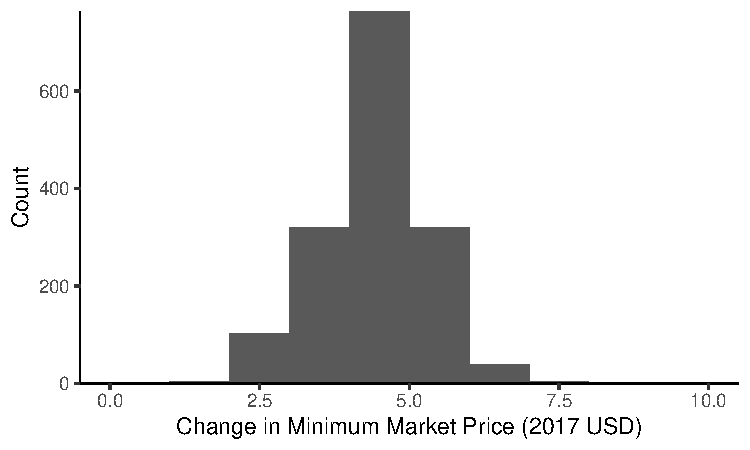
\includegraphics[width = 3.75in]{Merger_Change_MinimumFare_BestCase.pdf}
	\end{frame}
		
	\begin{frame}
			\frametitle{Merger Simulation Results: Minimum Fare}
			\framesubtitle{Average Marginal Cost}
			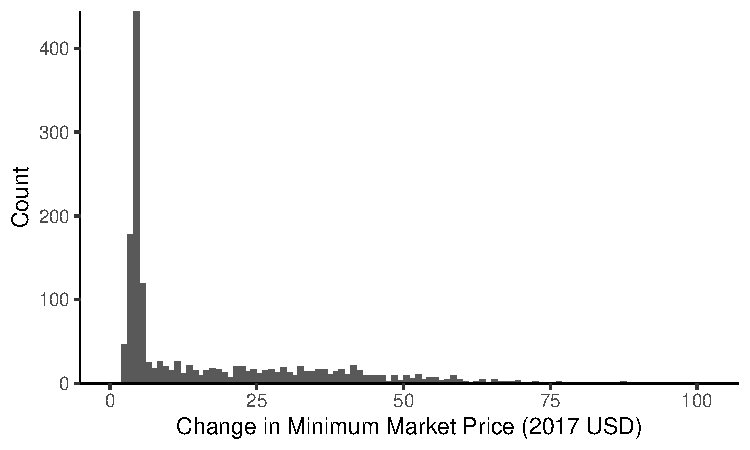
\includegraphics[width = 3.75in]{Merger_Change_MinimumFare_AverageCase.pdf}
		\end{frame}
		
		\begin{frame}
			\frametitle{Merger Simulation Results: Minimum Fare}
			\framesubtitle{Greatest Marginal Cost}
			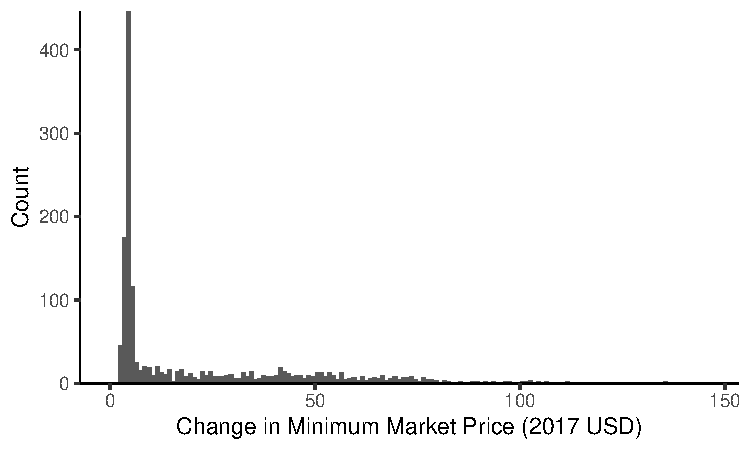
\includegraphics[width = 3.75in]{Merger_Change_MinimumFare_WorstCase.pdf}
       \end{frame}	
       	
       		\begin{frame}
       		\frametitle{Merger Simulation Results: Average Fare}
       		\framesubtitle{Lowest Marginal Cost}
       	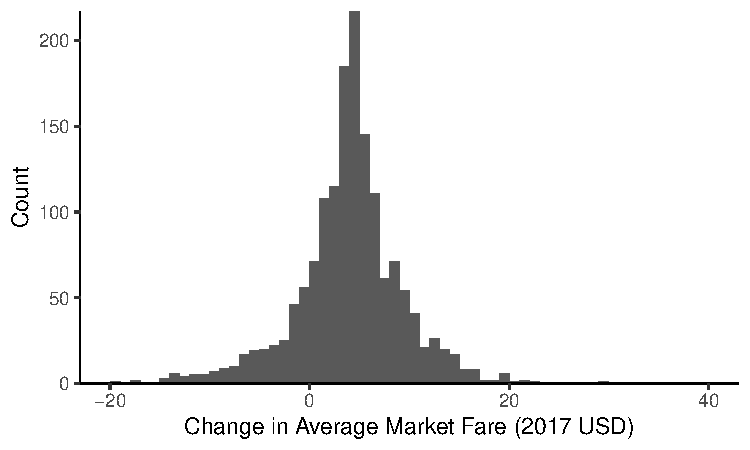
\includegraphics[width = 3.75in]{Merger_Change_AverageFare_BestCase.pdf}
       	\end{frame}
       	
       	\begin{frame}
       		\frametitle{Merger Simulation Results: Average Fare}
       		\framesubtitle{Average Marginal Cost}
       		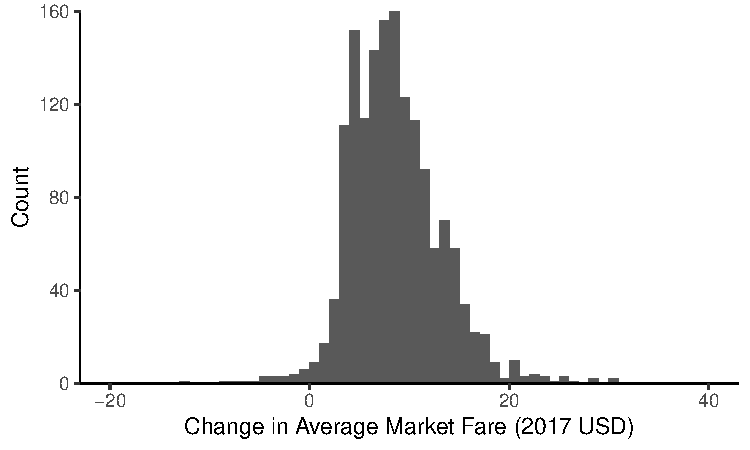
\includegraphics[width = 3.75in]{Merger_Change_AverageFare_AverageCase.pdf}
       	\end{frame}
       	
       	\begin{frame}
       		\frametitle{Merger Simulation Results: Average Fare}
       		\framesubtitle{Greatest Marginal Cost}
       	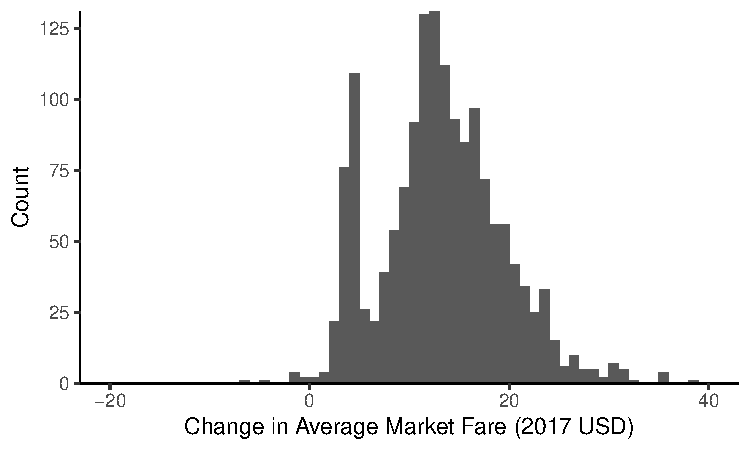
\includegraphics[width = 3.75in]{Merger_Change_AverageFare_WorstCase.pdf}
       	\end{frame}	
       	
	\section{Conclusion}
	\begin{frame}
		\frametitle{Conclusion}
		\begin{itemize}
			\item Minimum [Average] Market Fares in JetBlue-Spirit Markets Would have Increased by:
			\begin{itemize}
				\item Best Case: 4.47 [3.90]
				\item Average Case: 17.82 [8.51]
				\item Worst Case: 22.80 [13.18]
			\end{itemize}
			\item In the average JetBlue-Spirit market under the average cost scenario, customers would have paid \$876,000 more following the merger. 
		\end{itemize}
	\end{frame}

	\bibliography{airline}
	\bibliographystyle{abbrvnat.bst}
	
	
\end{document}


